\documentclass{article}
\usepackage{graphicx}
\usepackage{amsmath}
\usepackage{hyperref}
\usepackage{geometry}
\usepackage{setspace}
\doublespacing
\geometry{a4paper, margin=1in}
\title{Voice2Query: AI-Powered Speech-to-SQL for Interactive Database Exploration}

\author{Giovanni Fierro, Marco Apuzzo, Stefania Rosciano, Belal Hmeidat}
\date{\today}
\begin{document}
\begin{titlepage}
    \centering
    
    
\includegraphics[width=0.4\textwidth]{assets/unina_logo.jpeg}
    
    \vspace*{1cm}
    \Huge
    \textbf{Voice2Query: AI-Powered Speech-to-SQL for Interactive Database Exploration}

    \vspace{1cm}
    \Large{Fundamentals of Programming and Data Management}

    \vspace{1cm}
    \Large{Vincenzo Moscato}

    \vfill
    Keywords: WrenAI, Speechmatics, WhisperAI, Speech-to-Text, SQL DB, Natural Language Processing, Ollama

    \vfill
    \LARGE
    Giovanni Fierro, Marco Apuzzo, Stefania Rosciano, Belal Hmeidat
    
    \normalsize
    \vspace{1cm}
    \today
\end{titlepage}

\pagenumbering{roman}

\tableofcontents
\pagebreak
\listoffigures
\listoftables

\pagebreak
\pagenumbering{arabic}

\section{Introduction}
The \textbf{Voice2Query} project focuses on the design and implementation of a Speech-to-SQL pipeline, developed to allow users to interact with a relational database using spoken natural language.

The main goal is to break down the technical and syntactic barriers related to SQL knowledge for non-expert users, providing an intuitive and immediate access interface. The system captures voice input through a dedicated graphical interface, transcribes it into text, translates the text into a correct SQL query consistent with the database, and finally displays the results on an interactive dashboard.

To start the project, we needed to create a database to work with. We created a PostgreSQL database containing 3 tables with information about games, gamers, and reviews they gave to games.  Figure \ref{db_schema_fig} illustrates the database schema, showing the relationships between the tables and the fields contained in each table. The database was populated with synthetic data.

\begin{figure}[h!]
\begin{center}
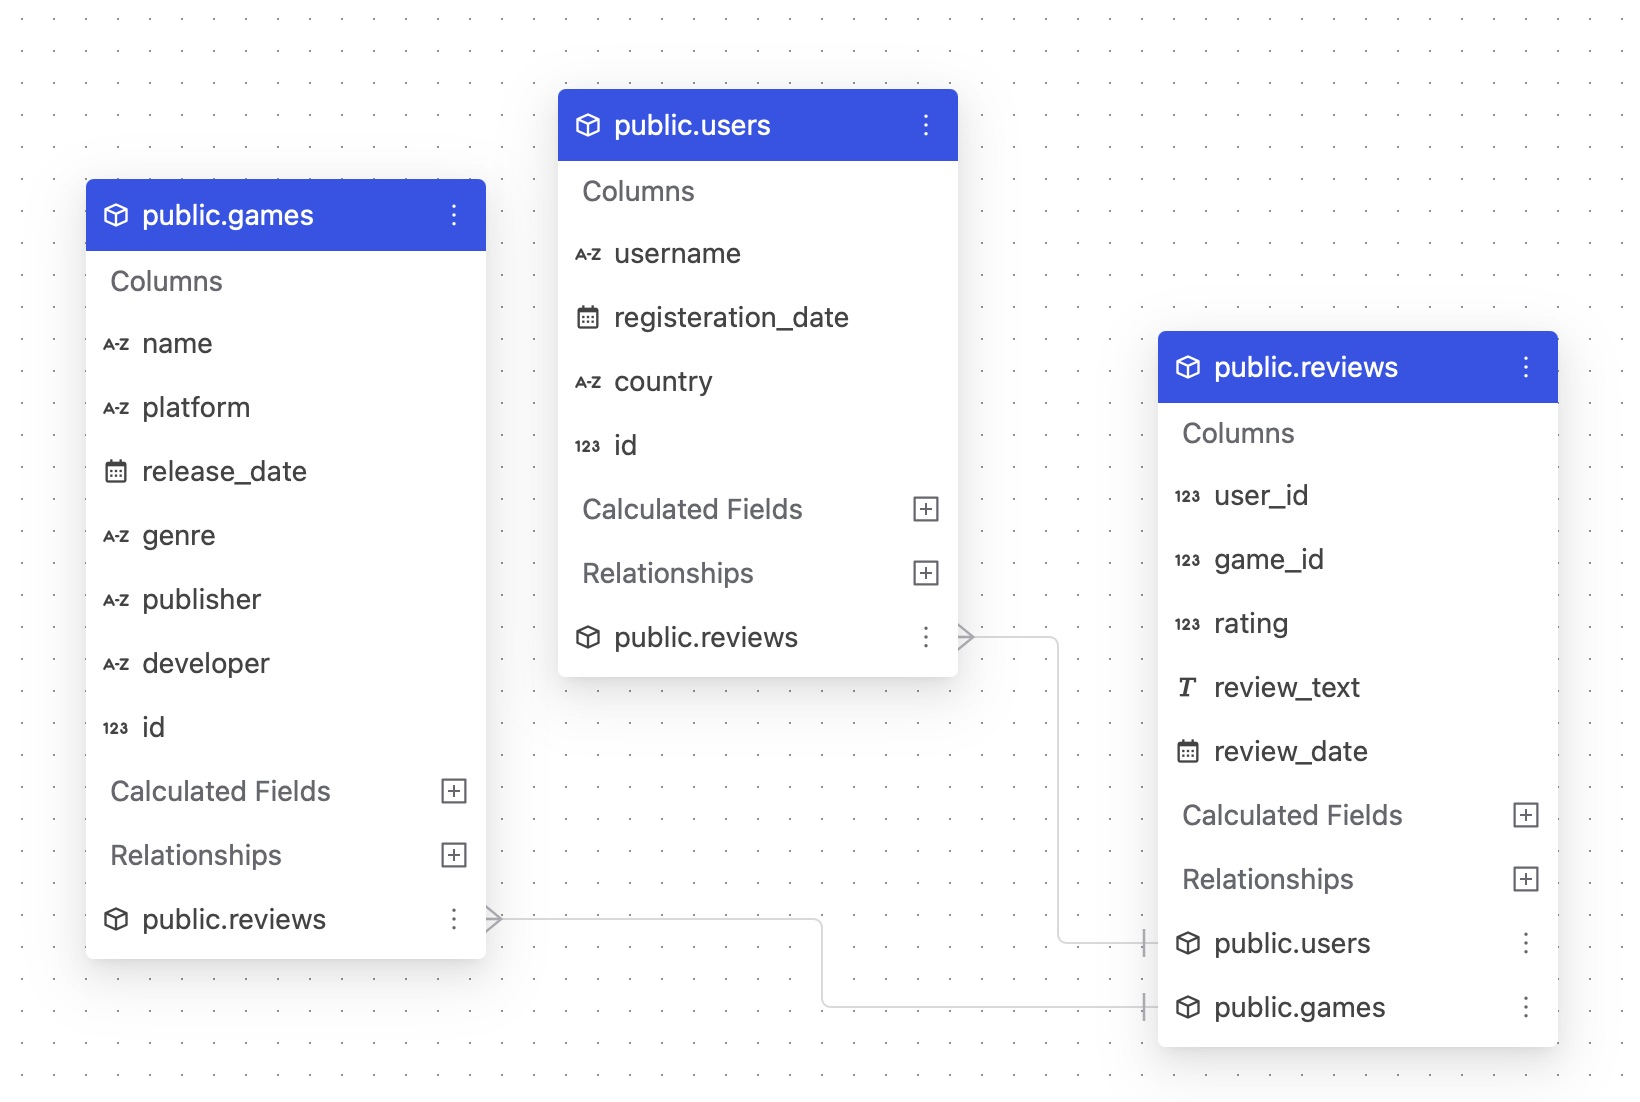
\includegraphics[width=0.8\textwidth]{assets/database_schema.jpeg}
\caption{Database Schema}
\label{db_schema_fig}
\end{center}
\end{figure}


\subsection{General System Architecture}
The system is based on a cascaded pipeline architecture, widely validated in scientific literature as a modular alternative to pure end-to-end models. To ensure service isolation, environment reproducibility, and infrastructure portability, the core of the pipeline was engineered through a hybrid Docker containerized and non containerized configuration. The network topology of the project involves a clear separation between core services and the client interface and is composed of 4 main components: the user interface, the FastAPI backend, the WrenAI container, and the DBMS container. Each component is designed to perform specific functions while maintaining clear communication channels with the others, ensuring a seamless user experience. Figure \ref{sys_arch_fig} illustrates the overall architecture of the system, highlighting the interactions between the different components and the flow of data.

\begin{figure}[h!]
\begin{center}
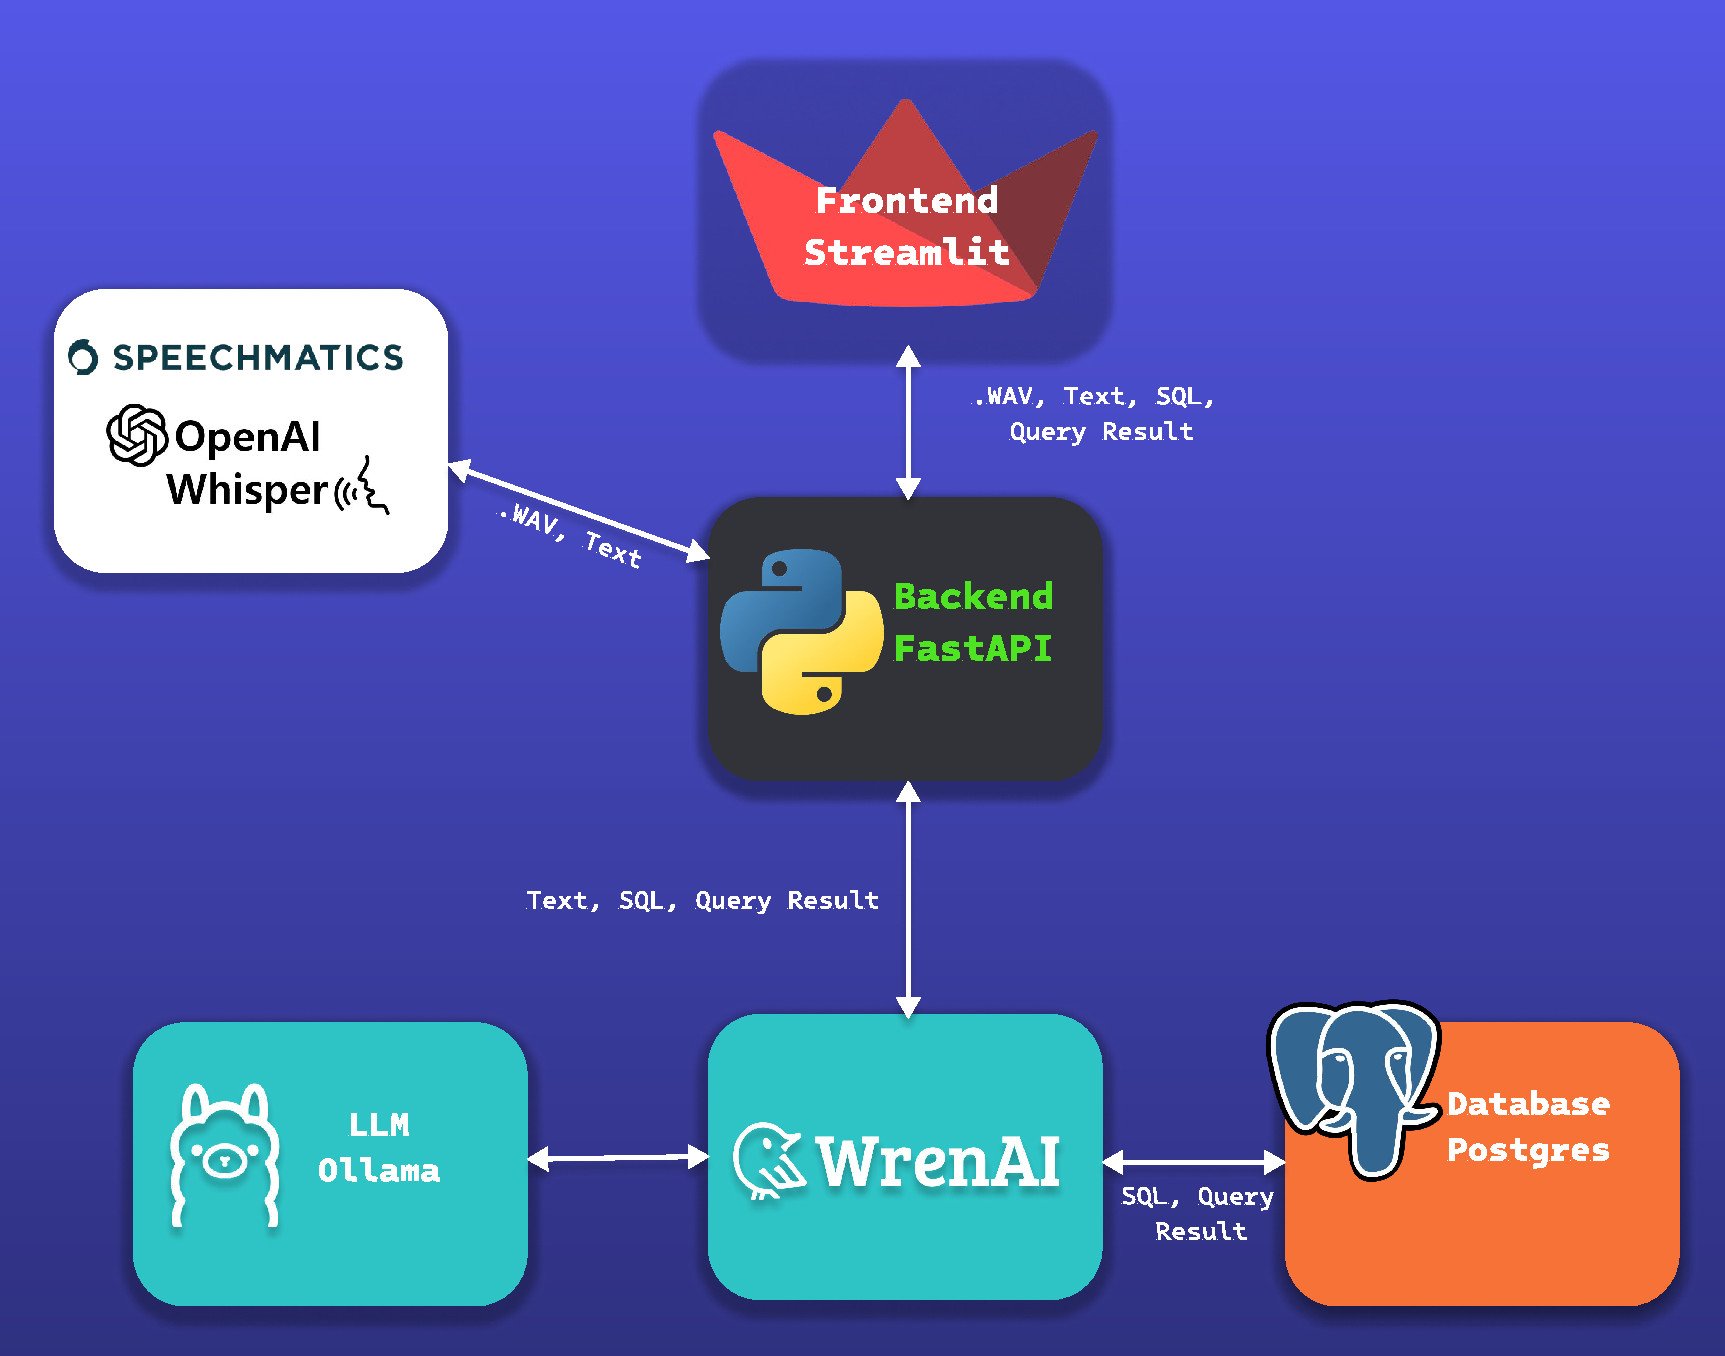
\includegraphics[width=0.8\textwidth]{assets/speech_to_SQL_diagram.pdf}
\caption{System Architecture Diagram}
\label{sys_arch_fig}
\end{center}
\end{figure}

The following describes each component in more detail:


\subsubsection{FastAPI Backend}
The FastAPI backend serves as the central hub for processing user requests. It separates the user interface 
from WrenAI and the database, ensuring that the system remains modular and maintainable. All communications from and to the backend The backend are done with RestAPI. The backend is responsible for receiving audio files from the client in the .wav format, forwarding them to the speech-to-text module: Speechmatics or Whisper, then sending the transcribed text to WrenAI for SQL query generation, executing the generated SQL query on the database, and finally sending the results back to the client for visualization.

\subsubsection{WrenAI Container (WrenAI Engine \& Configuration Console / WrenAI UI)}
This module runs the WrenAI engine. It houses both the logical back-end (which communicates with remote LLMs and the database) and its WrenAI UI (the Configuration Console). The latter is used exclusively during the development phase for establishing connection with the database, indexing, and semantically mapping the database metadata.

\subsubsection{DBMS Container (PostgreSQL)}
Hosts the active instance of the relational database. It is accessed by the WrenAI service and  and runs within an isolated Docker container, remaining shielded from unauthorized external access.

\subsubsection{User Interface (Streamlit)}
The main client application runs natively on the host machine. This choice is driven by the need to interface directly with local hardware peripherals for audio capture (microphone) and to maximize the responsiveness of the graphical dashboard during chart rendering. Streamlit communicates with the the backend through REST API calls, sending audio data, transcription, and receiving queries, and results for visualization.

\subsubsection*{Ollama}
To ensure the computational sustainability of the project, it was decided to exclude Ollama from the local Docker stack. The computationally intensive processes related to SQL code generation are delegated to enterprise-class Large Language Models accessible via external cloud APIs. This architectural design decision avoids overloading the local RAM and GPU VRAM, allowing the entire stack to run smoothly even on standard hardware architectures (such as thin clients or laptops without dedicated GPUs).

\section{Whisper AI v. Speechmatics}
\subsection{Transcription Accuracy}
We tested both models with sample text we read and recorded in clear English, and both models performed well with few errors. The test shows WhisperAI performing better on both WER and CER speech-to-text metrics, with approximately a 45\% improvement in WER. However, it should be noted that our tests aren’t comprehensive since they don’t evaluate the models with different languages, dialects, or noise levels. 
\subsection{Latency}
Another aspect to consider when considering the two solutions is the latency and live transcribing availability. Speechmatics supports real-time transcription, whereas WhisperAI works with batch processing of audio, which increases the time needed to transcribe in case of large audio files. 

\subsection{Hardware and Software Requirements}
The two tools have different requirements as Whisper AI gets installed locally and runs on the device or a private server. On the other hand, Speechmatics is a cloud-based service that saves the user a lot of resources.
\subsection{Ease of Integration}
Speechmatics, being a cloud-based solution, requires only API integration. WhisperAI, on the other hand, runs locally, which is good for offline workflow but makes any dependent package very large in size. Another option is to send requests to a dedicated private server running WhiserAI, but this requires maintaining additional servers, which in turn makes the integration process harder. However, Speechmatics might turn out to be more expensive in the long run than WhisperAI, as it is sold as a service, whereas WhisperAI is open source and free to utilize. 

\subsection{Multilingual Support}
Speechmatics supports 50+ languages, whereas WhisperAI supports 99 languages. This is probably due to the nature of the open nature of the WhisperAI project whereas Speechmatics is a proprietary service. However, the performance of both models on different languages requires futher testing.

\subsection{Speaker Diarization}
WhisperAI does not support speaker diarization natively. Instead, a community project called WhisperX adds this capability, utilizing the leading open-source solution provided by Pyannote. The open source version of Paynnote performs with an average Diarization Error Rate (DER) of 11.2\% \cite{whisperx_DER},so WhisperX is expected to perform similarly. On the other hand, Speechmatics supports speaker diarization natively, which is a significant advantage for users who require this feature. No public data is available on the performance of Speechmatics diarization, but it is expected to perform better than WhisperX since it is a paid service and not an open-source project.

\subsection{Comparison Table}
\begin{table}[h!]
\centering
\begin{tabular}{|l|c|c|}
\hline
\textbf{Feature} & \textbf{Whisper AI} & \textbf
{Speechmatics} \\
\hline
Transcription Accuracy & Very High & High \\
\hline
Live Transcription & Batches Only & Yes. Also supports batches \\
\hline
Hardware/Software Requirements & Local Installation & Cloud-Based \\
\hline
Ease of Integration & Moderate & Easy \\
\hline
Multilingual Support & 99+ Languages & 50+ Languages \\
\hline
Speaker Diarization & No (via WhisperX) & Yes \\
\hline

\end{tabular}
\caption{Comparison of Whisper AI and Speechmatics}
\end{table}

\subsection{Conclusion}
In conclusion, both Whisper AI and Speechmatics have their own strengths axnd weaknesses. Whisper AI excels in transcription accuracy and multilingual support, while Speechmatics offers real-time transcription and native speaker diarization. The choice between the two will depend on the specific needs of the user, such as the importance of real-time transcription, the need for speaker diarization, and budget constraints. For users who prioritize accuracy and multilingual support, Whisper AI may be the better choice. However, for those who require real-time transcription and native speaker diarization, Speechmatics may be more suitable.

In this project, we opted to use both solutions as they are both compatible with our architecture. The user is provided with an option in the UI to choose between the two solutions. 

\section{Text to SQL with WrenAI}
WrenAI is a powerful tool that allows for the translation of natural language queries into SQL code. It is designed to work with a variety of databases. The process of converting text to SQL with WrenAI involves several steps, including database indexing, semantic mapping, and query generation, all of which have been implemented in our project.

\subsection{Underlying Model}
We opted to use a legacy version Open Source of WrenAI that is free and runs locally on the machine to avoid WrenAI cloud service which costs money to use its tokens. This however requires coupling WrenAI with Ollama, which is a local Open Source LLM hosting solution. The WrenAI stack which includes WrenAI UI, engine, and service runs in a dedicated Docker container, while Ollama runs natively on the host machine to ensure optimal performance. The WrenAI engine is responsible for processing the transcribed text and generating the corresponding SQL queries, while the WrenAI UI is used for configuration and management of the WrenAI engine. The WrenAI service enables communication with the WrenAI engine using REST API calls, allowing for seamless integration with our FastAPI based backend. 

\subsection{Database Compatibility}
WrenAI supports a wide range of databases, including PostgreSQL, MySQL, and SQLite. In our project, we used PostgreSQL as our database management system since it is widely used in the industry and offers robust features for handling complex queries.

\subsection{Issues and Limitations}
Using the legacy version of WrenAI means that the accuracy of the generated SQL queries may not be as high as desired. We saw this in our testing, where some of the generated SQL queries were not correct and required manual correction. 
Correction can be done by the user through our custom UI to the transcribed text. 
Furthermore, needing to use Ollama to run the LLM locally adds more latency and accuracy issues since the LLMs that can be run locally are not as powerful as the ones available on the cloud. Nonetheless, using the local version of WrenAI and Ollama allows us to avoid the costs associated with using the cloud-based WrenAI service, making it a more cost-effective solution for our project.

\pagebreak
% \section*{References}
\begin{thebibliography}{9}
\bibitem{whisperx_DER}
Benchmarking Diarization Models, arxiv.org/html/2509.26177v1. Accessed 11 May 2026. 

\bibitem{speechmatics}
Speechmatics, ``Speechmatics Documentation,'' 2024.
\end{thebibliography}
\end{document}
